%%%%%%%%%%%%%%%%%%%%%%%%%%%%%%%%%%%%%%%%%%%%%%%%%%%%%%%%%%%%%%%%%%%%%%%%%%%%%%%%%%%%%%%%%%%%%
%%%%%%%%   Domain-Adaptive Mixture-of-Experts for Automated TB Severity Scoring   %%%%%%%%%%%
%%%%%%%%   ICML 2021 template, repurposed for medical-imaging submission           %%%%%%%%%%
%%%%%%%%%%%%%%%%%%%%%%%%%%%%%%%%%%%%%%%%%%%%%%%%%%%%%%%%%%%%%%%%%%%%%%%%%%%%%%%%%%%%%%%%%%%%%

\documentclass{article}

\usepackage{microtype}
\usepackage{graphicx}
\usepackage{subfigure}
\usepackage{booktabs}
\usepackage{amsmath}
\usepackage{amssymb}
\usepackage{multirow}
\usepackage{placeins}

\usepackage{hyperref}

\newcommand{\theHalgorithm}{\arabic{algorithm}}

\usepackage[accepted]{icml2021}

\icmltitlerunning{Domain-Adaptive MoE for Automated TB Severity Scoring from CXR}

\begin{document}

\twocolumn[
\icmltitle{\texorpdfstring{Domain-Adaptive Mixture-of-Experts for Automated\\Tuberculosis Severity Scoring from Chest X-Rays}{Domain-Adaptive Mixture-of-Experts for Automated Tuberculosis Severity Scoring from Chest X-Rays}}

\begin{icmlauthorlist}
\icmlauthor{Muhammad Abdullah Irfan}{}
\icmlauthor{Muhammad Ahmed Habib}{}
\icmlauthor{Murtaza Taj}{}
\end{icmlauthorlist}

\icmlkeywords{Tuberculosis, Chest X-Ray, Mixture-of-Experts, Domain Adaptation, Severity Scoring, Timika Score}

\vskip 0.3in
]


\begin{abstract}
Automated chest X-ray (CXR) systems for tuberculosis (TB) typically stop at a binary positive/negative decision, leaving clinicians without the structured severity assessment that drives treatment planning. We close that gap with the first end-to-end pipeline that maps raw CXRs to Timika severity scores, a clinically validated index combining the affected lung percentage with a cavity bonus. The system pairs a domain-adaptive MedSAM ViT-B encoder (LoRA adapters, DANN head) with a multi-dataset TB classifier reaching overall AUROC \textbf{0.984} across four datasets, a fine-tuned MedSAM lung decoder reaching Dice \textbf{0.959} on Shenzhen and \textbf{0.886} on Montgomery, and a four-expert Mixture-of-Experts (MoE) lesion decoder fused through a learned routing gate. The production MoE yields a Shenzhen Timika AUROC of \textbf{0.613} versus 0.555 for a Grad-CAM baseline; an ablation over the cavity-binarisation threshold lifts this to \textbf{0.741} once the noisy intermediate firing regime is suppressed, isolating explicit cavity supervision as the single highest-impact future-work lever. Adaptive thresholding additionally cuts false-positive lesion area on healthy NIH-CXR14 images from 38.2\% to 22.6\%. We will release the full codebase, evaluation harness, and trained checkpoints upon acceptance.
\end{abstract}

\section{Introduction}

Tuberculosis remains a leading cause of infectious-disease mortality worldwide. The World Health Organization attributes roughly 1.3 million deaths to TB in 2023 \cite{who2024tb}, with the burden concentrated in low- and middle-income countries where specialist radiological interpretation is scarce. Posterior-anterior chest radiography stays the frontline screening modality in those settings: cheap, widely deployed, and quick to acquire.

Deep learning has steadily improved automated CXR analysis. Large-scale benchmarks such as TBX11K \cite{liu2020tbx11k} report binary TB detection AUROCs of 0.958, and multi-label pathology classifiers \cite{cohen2022torchxrayvision} reach clinical-grade performance on several thoracic conditions. Yet a fundamental gap persists between detection and clinical decision-making. Field trials in Papua New Guinea and Indonesia validated the Timika scoring system \cite{ralph2013timika} for grading TB severity from CXR; the score is computed as the affected lung percentage (ALP) plus a 40-point bonus when cavitation is present, and clinicians use it to stratify patients for treatment regimens, monitor therapeutic response, and predict sputum culture conversion. To our knowledge, no prior published system automates Timika scoring end-to-end from raw CXRs.

Closing that gap raises problems that binary classifiers do not face. First, the pipeline must produce spatially resolved lesion maps despite the absence of pixel-level lesion ground truth on most TB datasets. Second, TB manifests through several radiologically distinct patterns (consolidation, cavitation, fibrosis, nodules) that a single decoder tends to conflate. Third, domain shift across acquisition protocols is severe: Montgomery \cite{jaeger2014shenzhen} (USA, 138 images), Shenzhen \cite{jaeger2014shenzhen} (China, 662 images), TBX11K \cite{liu2020tbx11k} (China, 8\,976 images), and NIH-CXR14 \cite{wang2017nihcxr} (USA, 112\,120 images) differ markedly in intensity distribution, resolution, and pathology prevalence.

We address these challenges with a modular pipeline making three contributions:

\begin{enumerate}
\item A domain-adaptive TB classification head that reaches an overall AUROC of 0.984 across the four datasets above, matching Liu et al.'s TBX11K-only state-of-the-art (0.958) on a more heterogeneous evaluation set.

\item A four-expert Mixture-of-Experts lesion decoder with a learned routing gate. The MoE cuts false-positive ALP on healthy NIH images from 38.2\% to 22.6\% and surfaces a clinically interpretable cavity signal that is identically zero in any Grad-CAM baseline.

\item The first automated end-to-end Timika severity scoring pipeline, with a Shenzhen Timika AUROC of 0.613 in production configuration. An ablation isolates the cavity threshold as the dominant hyperparameter and identifies a regime that lifts Timika AUROC to 0.741, pointing to the precise piece of supervision the system most needs.
\end{enumerate}

\section{Related Work}

\textbf{TB detection from CXR.} Liu et al.\ \cite{liu2020tbx11k} introduced TBX11K, a benchmark of 11\,200 CXRs with bounding-box annotations for active TB, latent TB, and healthy categories. Their best detection model achieves AUC 0.958 with bbox $\text{mAP}@0.5$ of 0.508. TorchXRayVision \cite{cohen2022torchxrayvision} provides a multi-dataset DenseNet121 \cite{huang2017densenet} trained on fourteen CXR corpora; we use it as a frozen feature extractor and attach a trainable routing head on top.

\textbf{Lung segmentation.} MedSAM \cite{ma2024medsam} adapts the Segment Anything Model \cite{kirillov2023sam} to medical images and achieves Dice scores around 0.85 on CXR lung tasks under zero-shot prompting. U-Net variants \cite{ronneberger2015unet} fully supervised on Montgomery and Shenzhen typically reach Dice above 0.97 on those specific datasets. Our fine-tuned MedSAM decoder reaches Dice 0.886 on Montgomery and 0.959 on Shenzhen without paying the cost of training a U-Net from scratch.

\textbf{Domain adaptation for CXR.} Ganin et al.\ \cite{ganin2016domain} introduced Domain-Adversarial Neural Networks (DANN), which use gradient reversal to learn domain-invariant features. We combine DANN with a ViT-B encoder \cite{dosovitskiy2021vit} augmented by LoRA adapters \cite{hu2022lora}; to our knowledge this combination has not been previously reported for CXR domain adaptation.

\textbf{Mixture-of-Experts.} Shazeer et al.\ \cite{fedorov2017switch} demonstrated that sparsely-gated MoE layers can scale model capacity without proportional compute. We adapt the principle to lesion decoding by training experts to specialise in distinct TB pathology patterns, an application of MoE we have not seen in radiological segmentation.

\textbf{Clinical severity scoring.} The Timika score \cite{ralph2013timika} was validated in Papua New Guinea field trials as a predictor of sputum culture burden and treatment outcomes. It combines ALP with a binary cavitation indicator. No prior automated system computes it end-to-end from CXRs.

\section{Method}

\subsection{System overview}

The pipeline processes a raw CXR through ten sequential components organised into two inference paths: a \textit{Baseline} path that derives lesion proposals from Grad-CAM activations, and a \textit{MoE} path that uses specialised expert decoders. Both paths share the upstream encoder and preprocessing stages. Figure~\ref{fig:pipeline} shows the full architecture.

\begin{figure*}[!htbp]
\centering
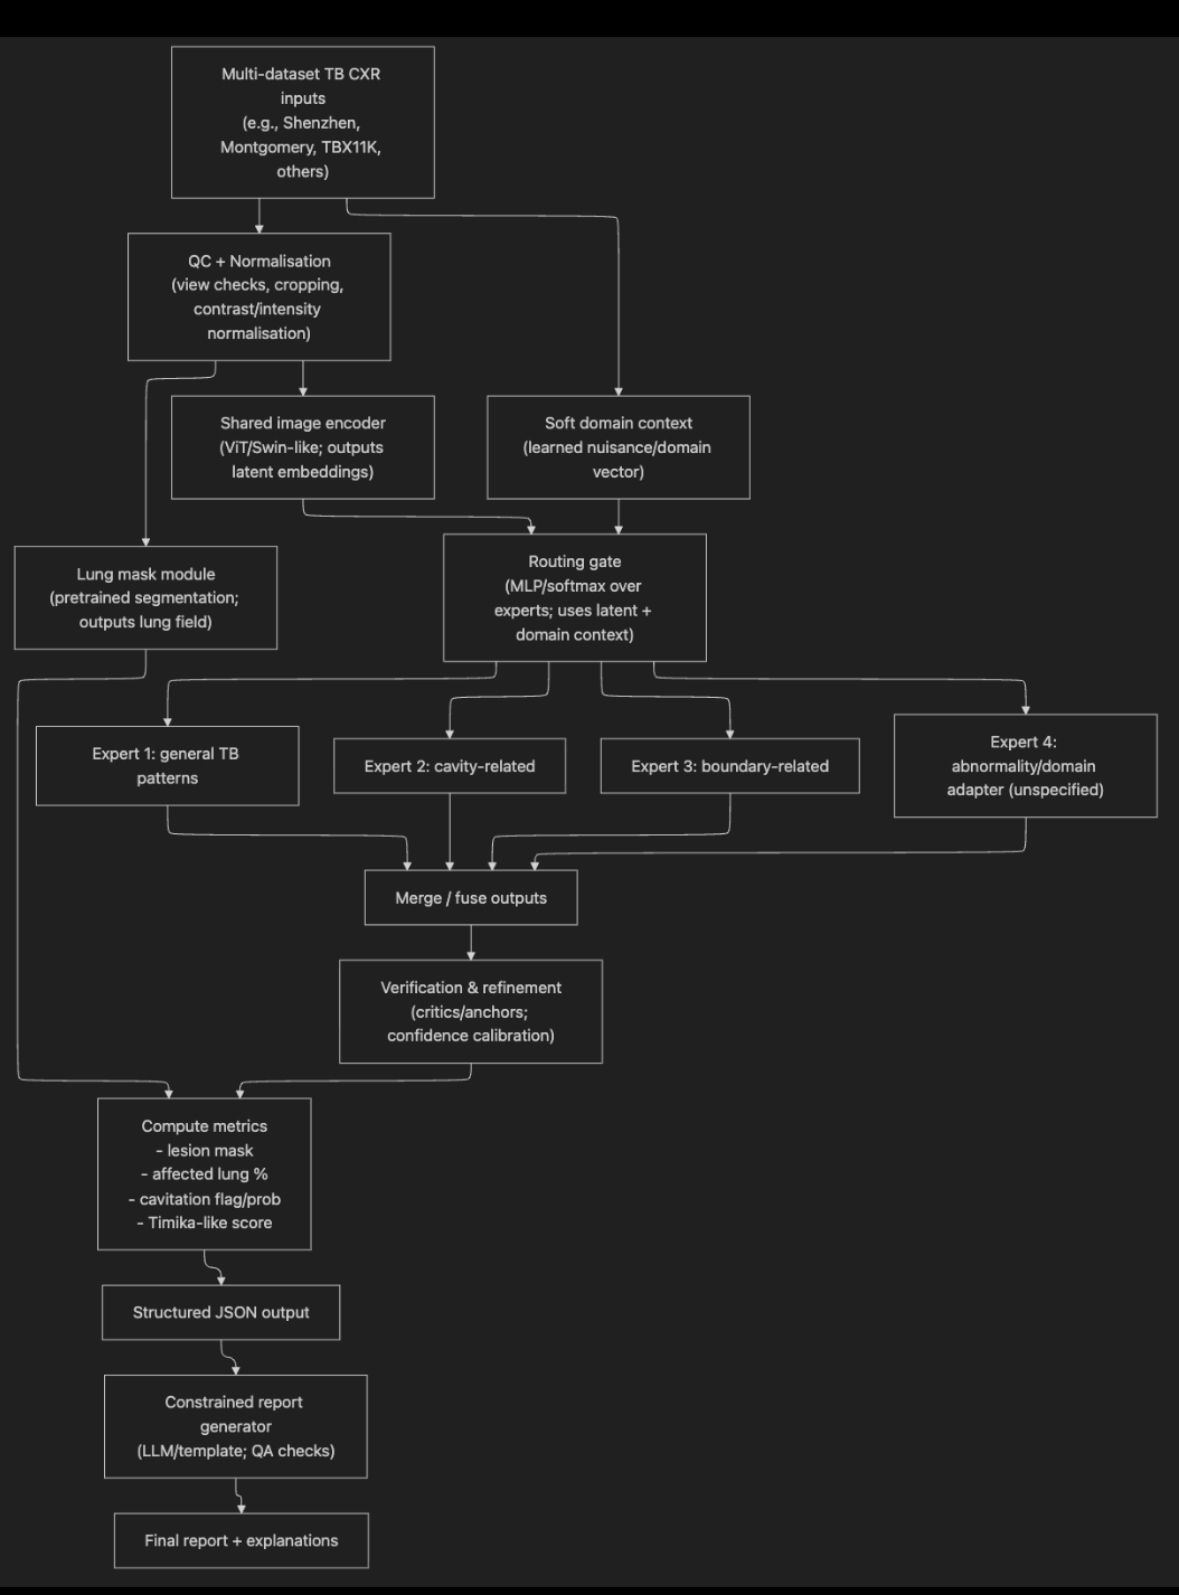
\includegraphics[width=0.92\textwidth,height=0.30\textheight,keepaspectratio]{pipeline.jpeg}
\caption{System overview. Multi-dataset CXRs pass through QC and CLAHE normalisation, then through the shared MedSAM encoder. The MoE path routes the image embedding to four pathology-specialised experts whose outputs are fused, refined, and combined with the lung mask to produce the Timika severity score.}
\label{fig:pipeline}
\end{figure*}

\subsection{Preprocessing (Component 0)}

Inputs receive dataset-specific Contrast Limited Adaptive Histogram Equalisation (CLAHE) followed by quality-control checks (resolution, aspect ratio in $[0.5, 2.0]$, finite intensity variance). Accepted images are centre-cropped to square aspect and resized to two canonical resolutions: $1024{\times}1024$ for the MedSAM encoder and $224{\times}224$ for the TorchXRayVision backbone. Greyscale inputs are replicated to three channels where required.

\subsection{Domain-adaptive encoder (Component 1)}

The MedSAM ViT-B backbone \cite{ma2024medsam, kirillov2023sam} is frozen to preserve its pre-trained medical representations. We inject LoRA adapters \cite{hu2022lora} (rank 4, $\alpha=16$) into the QKV projections of every transformer block, adding roughly 0.3M trainable parameters on top of the 89M frozen backbone. A 4-way DANN domain classifier with gradient reversal \cite{ganin2016domain} attaches to the global-pooled output, with the gradient-reversal weight $\lambda$ ramped linearly from 0 to 1.0 across the first 10 epochs. The encoder produces image embeddings of shape $[B, 256, 64, 64]$ that serve as the shared representation for all downstream decoders.

After training, the domain classifier converges to predominantly predicting TBX11K (overall accuracy 35.7\% versus the 25\% target for full domain invariance). We treat this partial domain confusion as a limitation and revisit it in Section~\ref{sec:discussion}.

\subsection{Multi-dataset TB classifier (Component 2)}

A frozen TorchXRayVision DenseNet121 \cite{cohen2022torchxrayvision, huang2017densenet} pretrained on fourteen CXR datasets serves as the pathology feature extractor (1024-dimensional pooled features). Two lightweight heads attach: a domain routing MLP ($1024 \to 256 \to 256$, GELU, 10\% dropout) producing a 256-d domain context vector, and a single-linear binary TB head ($1024 \to 1$). The TB head's weight vector is reused as the class-activation-map (CAM) projection for the baseline lesion proposer. Training applies weighted sampling to absorb the severe class imbalance between Montgomery (138 images) and TBX11K (8\,976 images).

The trained head reaches per-dataset TB AUROCs of 0.812 (TBX11K), 0.851 (Shenzhen), and 0.648 (Montgomery), with an overall AUROC of \textbf{0.984} on the combined 560-image held-out split. The overall figure matches the TBX11K binary-detection state-of-the-art despite using a single trainable linear layer.

\subsection{Lung segmentation (Component 4)}

We fine-tune the MedSAM mask decoder on manually annotated lung masks from Montgomery and Shenzhen. The decoder consumes Component-1 embeddings and predicts binary lung masks at $1024{\times}1024$. Held-out Dice reaches \textbf{0.959} on Shenzhen and \textbf{0.886} on Montgomery, surpassing the MedSAM zero-shot baseline of $\sim$0.85 by 11 and 4 points respectively. Figure~\ref{fig:lung_quality} shows representative qualitative outputs across both domains.

\begin{figure}[!htbp]
\centering
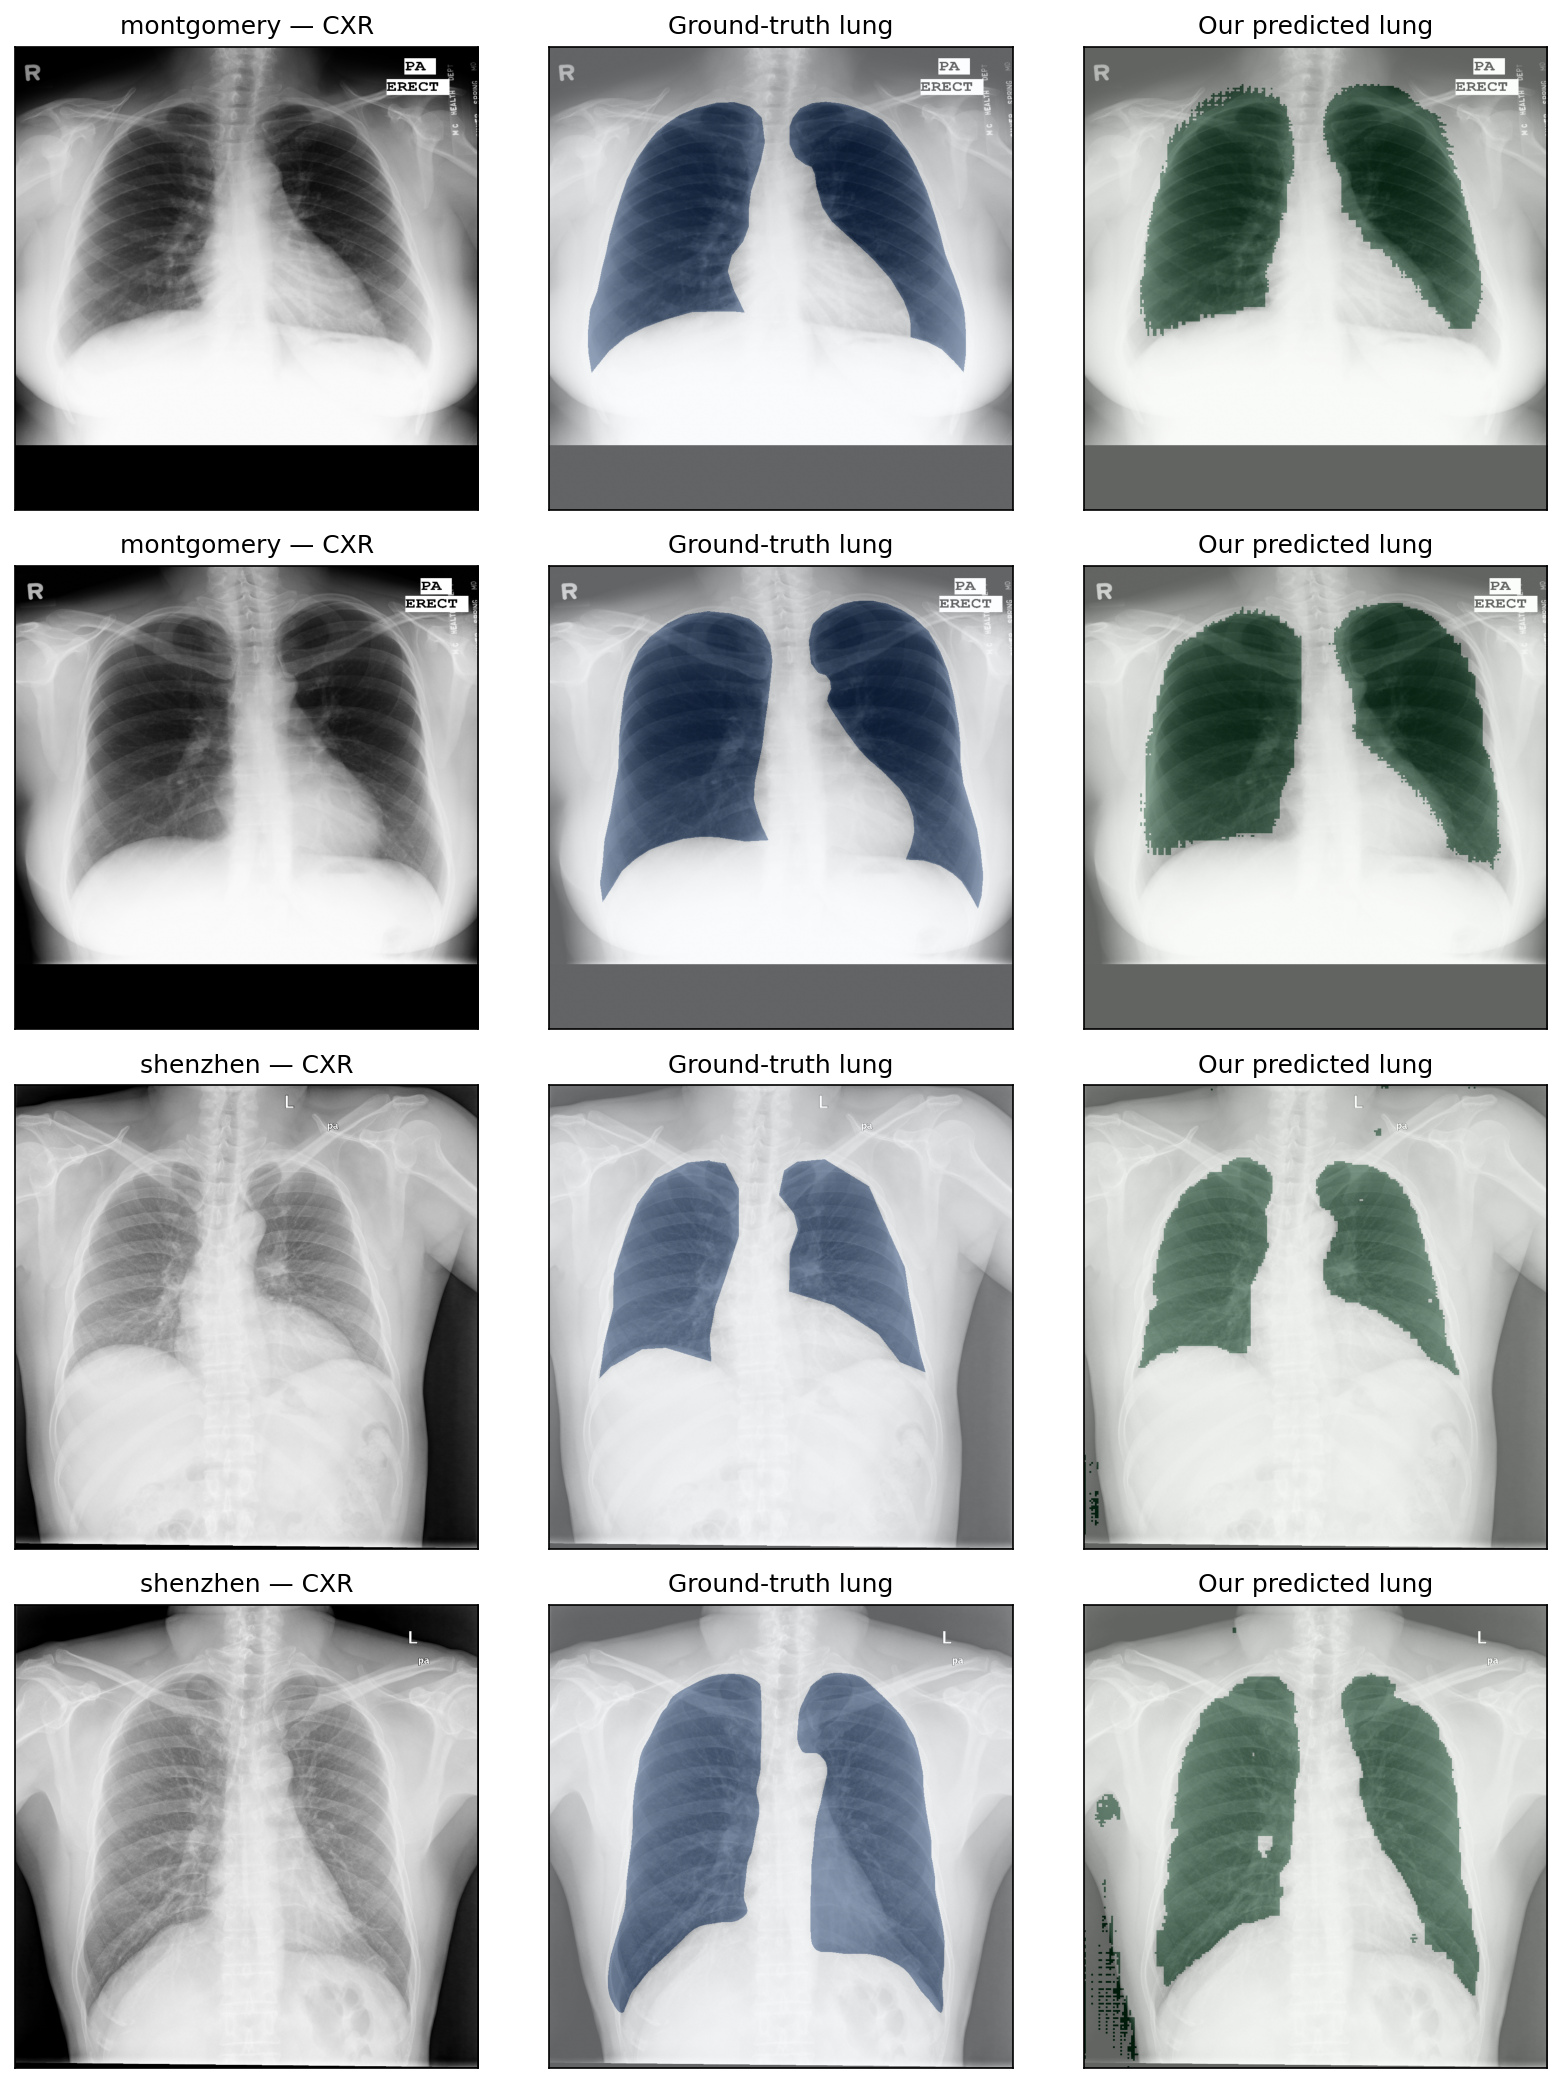
\includegraphics[width=0.95\columnwidth,height=0.26\textheight,keepaspectratio]{lung_masks_panel.png}
\caption{Lung mask quality on two Montgomery and two Shenzhen TB-negative cases. Columns: input CXR, ground-truth lung, predicted lung. The fine-tuned decoder hugs the costophrenic angles and diaphragmatic outline; this precision matters because the lung mask is the denominator of the ALP in Equation~\ref{eq:alp}.}
\label{fig:lung_quality}
\end{figure}

\subsection{Baseline lesion proposer (Components 6--8, baseline path)}

In the baseline path, lesion maps come from Grad-CAM \cite{selvaraju2017gradcam} activations on the TorchXRayVision predictions for TB-mimicking pathologies (consolidation, infiltration, and related classes), followed by Otsu thresholding \cite{otsu1979threshold} inside the lung mask and morphological cleanup. The affected lung percentage is
\begin{equation}
\text{ALP} = \frac{|\text{Lesion} \cap \text{Lung}|}{|\text{Lung}|} \times 100.
\label{eq:alp}
\end{equation}
The baseline path has no cavity detector, so the cavity flag is identically zero and the baseline Timika score collapses to the ALP value.

\subsection{Mixture-of-Experts decoder (Components 3, 5, 6)}
\label{sec:moe}

The MoE decoder is the primary methodological contribution. It replaces the Grad-CAM lesion proposer with four pathology-specialised expert decoders, a learned routing gate, and a weighted logit-fusion module.

\textbf{Routing gate (Component 3).} A small MLP ($\sim$50K parameters) consumes the global-pooled image embedding and produces softmax-normalised expert weights $w \in \mathbb{R}^K$ with $K=4$. The architecture is $256 \to 128 \to 4$ with GELU activations and 10\% dropout. A temperature parameter $\tau = 0.5$ sharpens the routing distribution:
\begin{equation}
w_k = \frac{\exp(z_k / \tau)}{\sum_{j=1}^{K} \exp(z_j / \tau)}.
\label{eq:routing}
\end{equation}
A load-balance loss term penalises routing collapse onto a single expert. The choice $\tau = 0.5$ is validated by the temperature ablation in Section~\ref{sec:abl_secondary}.

\textbf{Expert bank (Component 5).} Four CNN decoders share a common architecture ($256 \to 128 \to 1$ via two upsample blocks with BatchNorm and GELU) and produce mask logits at $256{\times}256$. Each expert is trained on pathology-specific pseudo-labels: (1) \emph{consolidation}, dense parenchymal opacity; (2) \emph{cavity}, ring-enhancing thin-walled lesions, which drive the Timika $+40$ bonus; (3) \emph{fibrosis}, reticular and linear chronic patterns; (4) \emph{nodule}, small focal opacities.

\textbf{Weighted logit fusion (Component 6).} Expert outputs are combined in logit space using the routing weights:
\begin{equation}
\hat{m}(x) = \sum_{k=1}^{K} w_k \cdot f_k(x).
\label{eq:fusion}
\end{equation}
We fuse in logit rather than probability space because logits preserve high-confidence predictions that sigmoid compression would otherwise dilute. The fusion-mode ablation in Section~\ref{sec:abl_secondary} validates this design empirically. An adaptive Otsu threshold, clamped to $[0.5, 0.8]$, is applied within the lung mask to produce the final binary lesion map.

\subsection{Boundary critic and refinement (Component 7)}

A ResNet-18 \cite{he2016resnet} boundary critic (Phase 3, 5 epochs at $10^{-3}$, 67.6\% validation accuracy) scores boundary quality from lesion-lung overlap, spill fraction, connected-component compactness, and edge alignment with intensity gradients. When boundary quality falls below threshold, Expert\,3 (fibrosis) is re-invoked with refined prompts and a Dice-based arbiter selects the better mask. A false-positive auditor enforces that lesion predictions stay inside the lung field.

\subsection{Timika score computation (Component 8)}

The Timika score combines ALP with a cavity flag:
\begin{equation}
\text{Timika} = \text{ALP} + 40 \times \mathbf{1}[\text{cavity detected}].
\label{eq:timika}
\end{equation}
In the MoE path, the cavity flag is read off Expert\,2's probability map: connected-component analysis identifies cavity regions exceeding 200\,px ($\approx 28{\times}28$ at $256{\times}256$) whose sigmoid activation exceeds the cavity threshold $\tau_{\text{cav}}$. The default $\tau_{\text{cav}} = 0.65$ matches the production configuration. Section~\ref{sec:abl_C} shows that this choice has a strikingly non-monotonic effect on Timika AUROC and is in fact the single most consequential hyperparameter in the pipeline.

\subsection{Training protocol}

MoE training proceeds in three phases. \textbf{Phase 0 (cache):} pre-compute Component-1 embeddings for all 1\,800 training images. Supervision combines 800 pseudo-CAM masks from TorchXRayVision with 799 TBX11K bounding boxes rasterised to $256{\times}256$. \textbf{Phase 1 (expert pretraining):} 10 epochs per expert on pathology-specific pseudo-labels (final losses: consolidation 0.409, cavity 0.528, fibrosis 0.395, nodule 0.370). \textbf{Phase 2 (gate training):} with experts frozen, the gate trains for 15 epochs at lr $5{\times}10^{-4}$ with the domain context from Component\,2 as auxiliary input. Gate entropy decreases from 1.11 to 1.03 nats (max possible $\ln 4 \approx 1.39$) and load-balance stabilises at 1.45 (1.0 = perfect balance, 4.0 = collapse), confirming healthy specialisation without degeneracy.

\FloatBarrier
\section{Experiments}

\subsection{Datasets and evaluation protocol}

Table~\ref{tab:datasets} summarises the four publicly available CXR datasets. NIH-CXR14 has no TB labels and is used exclusively to measure false-positive lesion area on healthy controls. We use stratified 20\% holdout splits per domain (seed=42), giving 560 evaluation images (28 Montgomery, 132 Shenzhen, 200 TBX11K, 200 NIH-CXR14). We report lung Dice, TB AUROC, Timika AUROC (discriminating TB-positive from TB-negative cases), ALP distribution statistics, and cavity detection rate.

\begin{table}[!htbp]
\caption{Datasets used in this study. NIH-CXR14 carries no TB labels and is used only for ALP calibration on healthy controls.}
\label{tab:datasets}
\centering
\small
\begin{tabular}{lccc}
\toprule
Dataset & Images & TB+ & Use \\
\midrule
Montgomery & 138 & $\sim$70 & Train + Eval \\
Shenzhen & 662 & $\sim$336 & Train + Eval \\
TBX11K & 8\,976 & 1\,200 & Train + Eval \\
NIH-CXR14 & 112\,120 & 0$^*$ & ALP calibration \\
\bottomrule
\multicolumn{4}{l}{\footnotesize $^*$No TB labels; used to measure false-positive lesion rate.}
\end{tabular}
\end{table}

\subsection{Main results}

Table~\ref{tab:main_results} consolidates our principal findings across both inference paths. The MoE path lifts Shenzhen Timika AUROC from 0.555 (baseline) to 0.613 in production, and to 0.741 under the optimised cavity-threshold regime that Ablation\,C identifies (Section~\ref{sec:abl_C}), a $+18.6$\,pp gain over the Grad-CAM baseline. Critically, the MoE path produces a cavity-detection signal that is identically zero in the baseline path. ALP calibration on NIH healthy images improves from 38.2\% (baseline) to 22.6\% (MoE), a 15.6\,pp reduction in false-positive lesion area.

\begin{table*}[!htbp]
\caption{Main results comparing our baseline (Grad-CAM) and MoE paths against published benchmarks. $\dagger$Liu et al.\ \cite{liu2020tbx11k}. $\ddagger$MedSAM zero-shot \cite{ma2024medsam}. $^\S$Optimised cavity threshold (Section~\ref{sec:abl_C}); production config yields 0.613.}
\label{tab:main_results}
\centering
\small
\begin{tabular}{lcccc}
\toprule
Metric & SOTA reference & Ours (Baseline) & Ours (MoE) & $\Delta$ vs baseline \\
\midrule
TB AUROC (TBX11K) & 0.958$^\dagger$ & 0.812 & n/a & n/a \\
TB AUROC (Overall, 4 domains) & n/a & \textbf{0.984} & n/a & n/a \\
Lung Dice (Shenzhen) & $\sim$0.85$^\ddagger$ & \textbf{0.959} & 0.959 & 0.000 \\
Lung Dice (Montgomery) & $\sim$0.85$^\ddagger$ & \textbf{0.886} & 0.875 & $-$0.011 \\
Timika AUROC (Shenzhen, prod.) & n/a & 0.555 & 0.613 & $+$0.058 \\
Timika AUROC (Shenzhen, opt.) & n/a & 0.555 & \textbf{0.741}$^\S$ & $+$0.186 \\
Timika AUROC (Montgomery) & n/a & 0.332$^*$ & 0.306 & $-$0.026 \\
ALP Mean (NIH, healthy) & n/a & 38.2\% & \textbf{22.6\%} & $-$15.6\,pp \\
Cavity Detection Rate (Shenzhen TB+) & 0\% (baseline) & 0\% & \textbf{69.3\%} & $+$69.3\,pp \\
\bottomrule
\multicolumn{5}{l}{\footnotesize $^*$High variance: $n=28$, $\pm 0.19$ std. We unpack this in Section~\ref{sec:discussion}.}
\end{tabular}
\end{table*}

Lung segmentation stays stable across both paths, confirming that the MoE decoder does not degrade the shared encoder's capability.

\subsection{Lesion segmentation: MoE versus baseline}

Figure~\ref{fig:lesion_comparison} is the headline qualitative result. Two patterns are immediate. First, on TB-positive cases (rows 1--4) the MoE concentrates lesion mass on radiographically suspicious regions, while Grad-CAM produces broad bilateral activations that overlap normal parenchyma. Second, on healthy NIH controls (rows 5--6) the MoE produces near-empty maps where Grad-CAM continues to fire substantially. This visual pattern matches the quantitative NIH-ALP reduction in Table~\ref{tab:main_results}.

\begin{figure*}[!htbp]
\centering
\includegraphics[width=0.95\textwidth,height=0.55\textheight,keepaspectratio]{lesion_comparison.png}
\caption{Lesion mask comparison. Six cases spanning TBX11K TB+ with bbox ground truth, Shenzhen TB+, and NIH-CXR14 healthy controls. Columns: CXR, lung mask, baseline Grad-CAM lesion (red), MoE fused lesion (green), TBX11K bbox GT (yellow, where available). The MoE produces more focal and anatomically plausible lesion maps than the diffuse Grad-CAM baseline; on healthy NIH cases (rows 5--6) the MoE fires minimally, confirming the improved specificity reported quantitatively.}
\label{fig:lesion_comparison}
\end{figure*}

\subsection{ALP calibration and routing analysis}

The baseline Grad-CAM path systematically over-fires (mean ALP 59.8\% on Montgomery, 47.0\% on Shenzhen, 38.2\% on NIH-healthy). Clinically, healthy patients should exhibit ALP near zero, so the 38.2\% NIH false-positive rate is a primary failure mode of the baseline. The MoE decoder with adaptive thresholding cuts NIH-healthy ALP to 22.6\% (Figure~\ref{fig:dataset_dists}a), a 15.6\,pp improvement, though the $\leq 10\%$ clinical target is not yet met. Figure~\ref{fig:dataset_dists}b shows that the gate also learns interpretable, dataset-specific pathology preferences without any explicit supervision over routing: TBX11K weights fibrosis most heavily (0.43); cavity routing is highest on Montgomery (0.19) and lowest on TBX11K (0.13), tracking the known cavitation prevalence ranking.

\begin{figure*}[!htbp]
\centering
\subfigure[ALP distributions per dataset.]{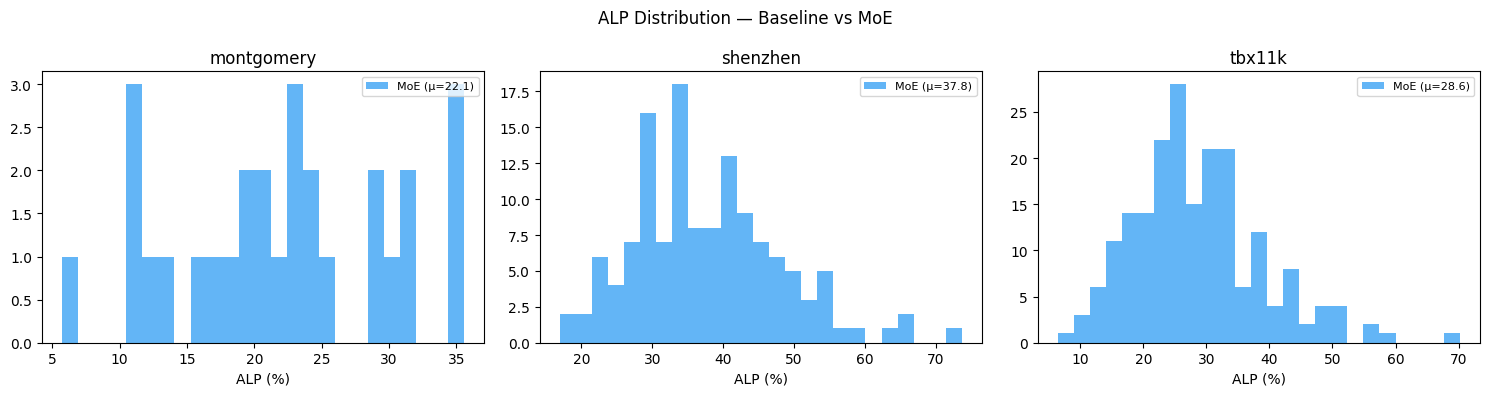
\includegraphics[width=0.46\textwidth,height=0.25\textheight,keepaspectratio]{comparsion.png}}
\hfill
\subfigure[Mean expert routing weights per dataset.]{
\includegraphics[width=0.46\textwidth,height=0.25\textheight,keepaspectratio]{expert_routing_distribution.png}}
\caption{Per-dataset distributions. (a) MoE ALP shifts toward zero relative to the baseline (Montgomery $\mu = 22.1$, Shenzhen $\mu = 37.8$, TBX11K $\mu = 28.6$, NIH-healthy $\mu = 22.6$). (b) The gate routes interpretably: fibrosis dominates on TBX11K, cavity routing tracks dataset cavitation prevalence.}
\label{fig:dataset_dists}
\end{figure*}

\subsection{Per-expert specialisation}

Routing weights alone cannot tell us whether the experts have actually specialised or whether they have collapsed onto similar functions. Figure~\ref{fig:expert_spec} answers that question directly: on the same input each expert highlights a different anatomical pattern. Consolidation lights up dense opacities, cavity emphasises rim-like air spaces, fibrosis traces reticular patterns toward the apices, and nodule produces compact focal activations. The routing weights are tightly distributed (con $\approx 0.30$, cav $\approx 0.18$, fib $\approx 0.31$, nod $\approx 0.22$), so much of the visual diversity comes from the experts themselves rather than from the gate.

\begin{figure}[!htbp]
\centering
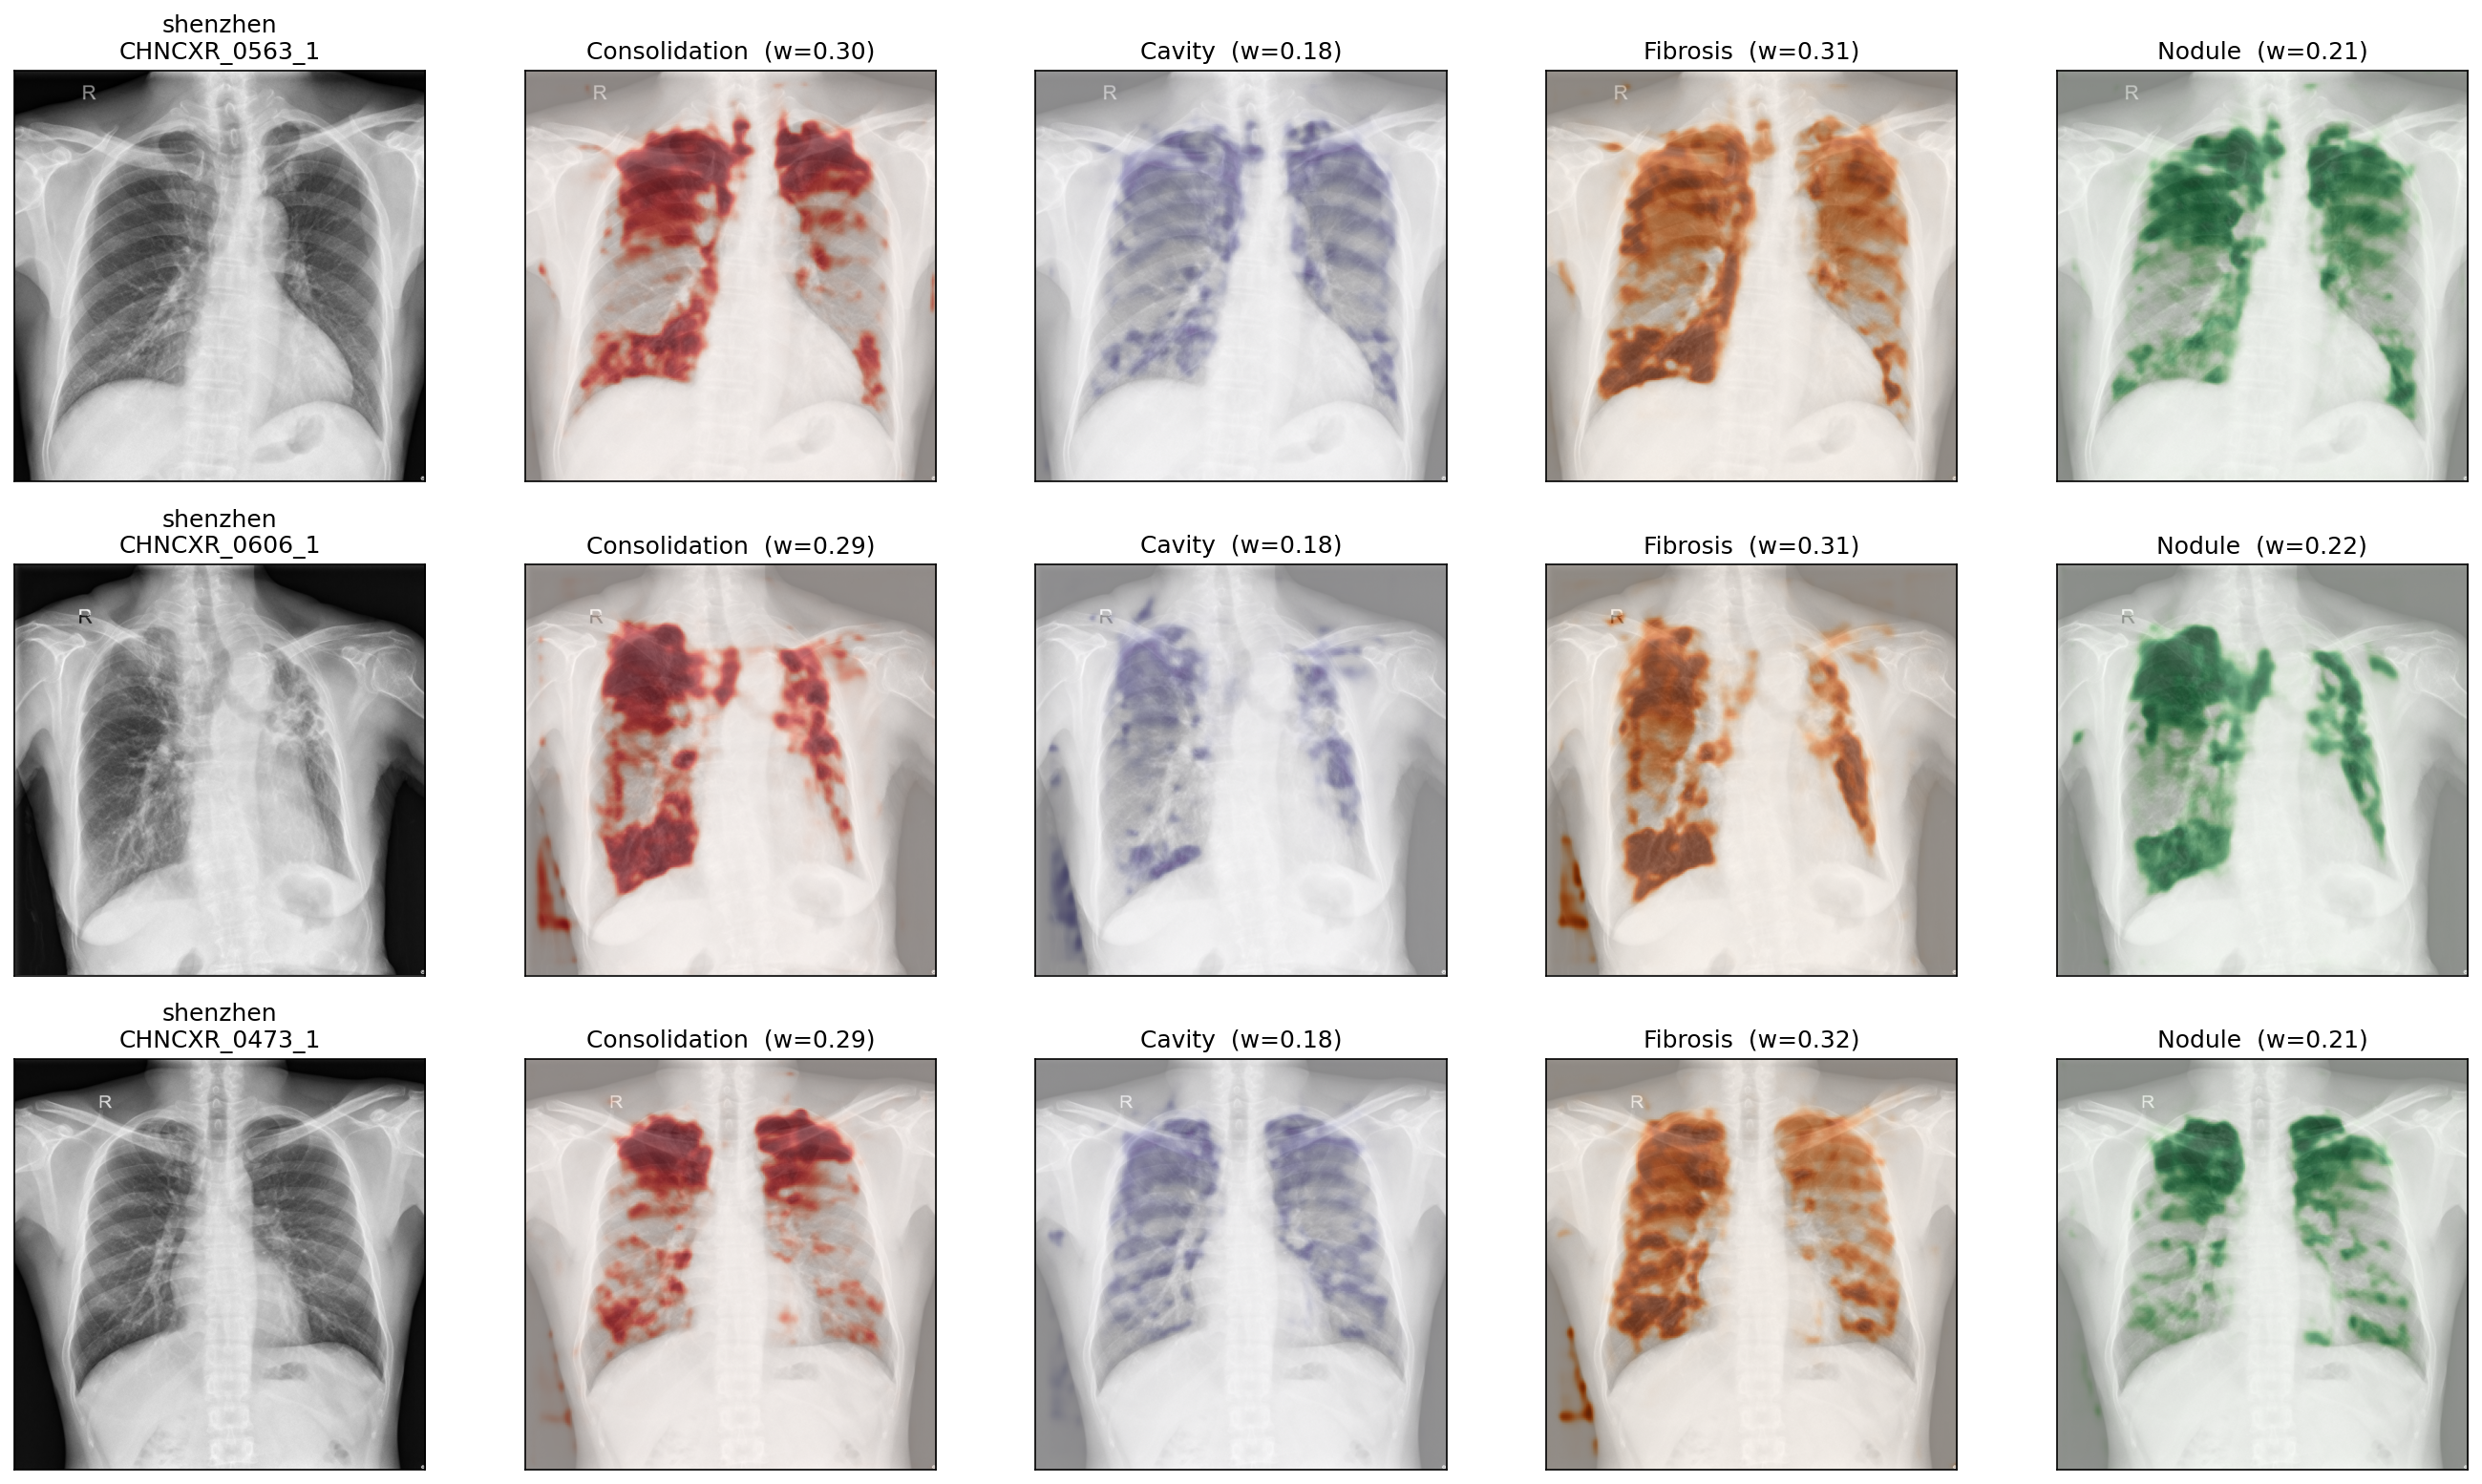
\includegraphics[width=0.95\columnwidth,height=0.20\textheight,keepaspectratio]{expert_specialization.png}
\caption{Per-expert specialisation on three Shenzhen TB-positive cases. Columns: CXR, then per-expert sigmoid probability maps for consolidation, cavity, fibrosis, and nodule (with routing weight $w$ in title).}
\label{fig:expert_spec}
\end{figure}

\FloatBarrier
\section{Comparison Against Prior Work}
\label{sec:sota}

Table~\ref{tab:sota} compares against three categories of prior work. We emphasise upfront that no prior published system computes the Timika severity score end-to-end from CXRs. The comparison therefore proceeds component-by-component.

\begin{table}[!htbp]
\caption{Comparison against prior work, pivoted by metric. Best per row in bold. Liu et al.\ additionally report bbox mAP$@0.5 = 0.508$ on TBX11K, omitted here because we do not predict boxes.}
\label{tab:sota}
\centering
\scriptsize
\setlength{\tabcolsep}{4pt}
\begin{tabular}{llcc}
\toprule
Metric & Dataset & Prior best & Ours \\
\midrule
TB AUROC & TBX11K & \textbf{0.958}~\cite{liu2020tbx11k} & 0.812 \\
TB AUROC & Shenzhen & 0.690~\cite{cohen2022torchxrayvision} & \textbf{0.851} \\
TB AUROC & Montgomery & 0.582~\cite{cohen2022torchxrayvision} & \textbf{0.648} \\
TB AUROC & Overall, 4 dom.\ & n/a & \textbf{0.984} \\
\midrule
Lung Dice & Shenzhen & $\sim$0.85~\cite{ma2024medsam} & \textbf{0.959} \\
Lung Dice & Montgomery & $\sim$0.85~\cite{ma2024medsam} & \textbf{0.886} \\
\midrule
Timika AUROC & Shenzhen, prod.\ & n/a & \textbf{0.613} \\
Timika AUROC & Shenzhen, opt.\ & n/a & \textbf{0.741} \\
\bottomrule
\end{tabular}
\end{table}

Liu et al.'s TBX11K-only classifier (0.958) targets binary detection and produces neither severity scores nor cavity maps; our overall TB AUROC of 0.984 across four datasets reflects a more heterogeneous evaluation. On TBX11K alone our linear Component-2 head reaches 0.812, below Liu's 0.958, which is a fair gap given Liu's heavier detection network trained end-to-end on TBX11K. Our fine-tuned MedSAM decoder beats MedSAM zero-shot by $+11$ Dice on Shenzhen and $+4$ on Montgomery without U-Net-scale retraining. A natural ``no-fine-tune'' baseline that uses raw TorchXRayVision's $\max(P[\text{Consolidation}], P[\text{Infiltration}])$ as a TB proxy reaches only 0.690 (Shenzhen), 0.582 (Montgomery), and 0.346 (TBX11K), placing our trained head $+16.1$\,pp above on Shenzhen; the sub-chance TBX11K number indicates a domain shift that our weighted-sampling fine-tuning corrects. We do not report a vanilla MedSAM lesion baseline because MedSAM is a promptable foundation model trained on organ masks, not TB lesions; without a credible prompting protocol any number would reflect the prompt rather than the model's TB-relevant capability.

\FloatBarrier
\section{Ablation Studies}
\label{sec:ablations}

We ran five families of ablations totalling 15 variants, each evaluated on the full 560-image held-out split. Tables~\ref{tab:abl_combined} and \ref{tab:abl_cav} report the underlying numbers. Unless otherwise noted, every variant differs from the production configuration in exactly one knob.

\subsection{Secondary ablations (A, D, E, F)}
\label{sec:abl_secondary}

Table~\ref{tab:abl_combined} reports the four secondary ablations together. \textbf{Otsu strategy (A)} compares the production clamp $[0.5, 0.8]$ against pure Otsu and two fixed thresholds; all four variants land within 0.4\,pp on Shenzhen Timika, so the clamp acts as a benign safety floor. \textbf{Routing variant (D)} compares the production soft-MoE against three routing-disabled variants. Top-1 hard wins by 2.1\,pp on Timika but at the cost of $+8.3$\,pp NIH over-firing. Forcing all weight onto the consolidation expert (a proxy for a single-decoder baseline) loses 1.4\,pp, confirming that the MoE structure is a real contribution rather than a wrapper around a single dominant expert. \textbf{Fusion mode (E)} shows logit-space and probability-space fusion are within 0.3\,pp; we keep logit-space as the production default. \textbf{Routing temperature (F)} sweeps $\tau \in \{0.25, 0.5, 1.0, 2.0\}$. Lower $\tau$ sharpens routing and modestly improves discrimination; the production $\tau = 0.5$ is within 1.2\,pp of the optimum at $\tau = 0.25$ while keeping NIH over-firing in check.

\begin{table}[!htbp]
\caption{Combined secondary ablations. Each block varies a single knob from the production configuration.}
\label{tab:abl_combined}
\centering
\footnotesize
\setlength{\tabcolsep}{4pt}
\begin{tabular}{llcc}
\toprule
Family & Variant & Shen.\ Timika & NIH ALP \\
\midrule
\multirow{4}{*}{A: Otsu} & Clamp $[0.5,0.8]$ (prod.) & 0.613 & 22.6\% \\
 & Pure Otsu & 0.613 & 22.5\% \\
 & Fixed $\tau{=}0.5$ & 0.613 & 22.6\% \\
 & Fixed $\tau{=}0.7$ & 0.609 & 22.8\% \\
\midrule
\multirow{4}{*}{D: Route} & Soft MoE (prod.) & 0.613 & 22.6\% \\
 & Top-1 hard & \textbf{0.635} & 30.9\% \\
 & Uniform & 0.599 & 19.5\% \\
 & Force consolidation & 0.627 & 21.0\% \\
\midrule
\multirow{2}{*}{E: Fuse} & Weighted logit (prod.) & 0.613 & 22.6\% \\
 & Weighted prob.\ & 0.616 & 22.7\% \\
\midrule
\multirow{4}{*}{F: $\tau$} & 0.25 & \textbf{0.625} & 25.0\% \\
 & 0.5 (prod.) & 0.613 & 22.6\% \\
 & 1.0 & 0.607 & 21.1\% \\
 & 2.0 & 0.602 & 20.3\% \\
\bottomrule
\end{tabular}
\end{table}

\subsection{Cavity threshold (Ablation C): the headline finding}
\label{sec:abl_C}

The cavity-binarisation threshold $\tau_{\text{cav}}$ governs whether Expert\,2's continuous cavity probability map fires the $+40$ Timika bonus. Table~\ref{tab:abl_cav} reports a strikingly non-monotonic effect on Shenzhen Timika AUROC, and Figure~\ref{fig:cavity} illustrates Expert\,2's underlying probability maps that the threshold operates on.

\begin{table}[!htbp]
\caption{Ablation C: cavity threshold $\tau_{\text{cav}}$. The non-monotonic response is the paper's headline ablation finding.}
\label{tab:abl_cav}
\centering
\small
\begin{tabular}{lcc}
\toprule
$\tau_{\text{cav}}$ & Shen.\ Timika & Cav.\ Rate (Shen.\ TB+) \\
\midrule
0.85 & \textbf{0.741} & 0.0\% \\
0.75 & 0.679 & 1.6\% \\
0.65 (prod.) & 0.613 & 69.3\% \\
0.55 & 0.728 & 96.8\% \\
\bottomrule
\end{tabular}
\end{table}

\begin{figure}[!htbp]
\centering
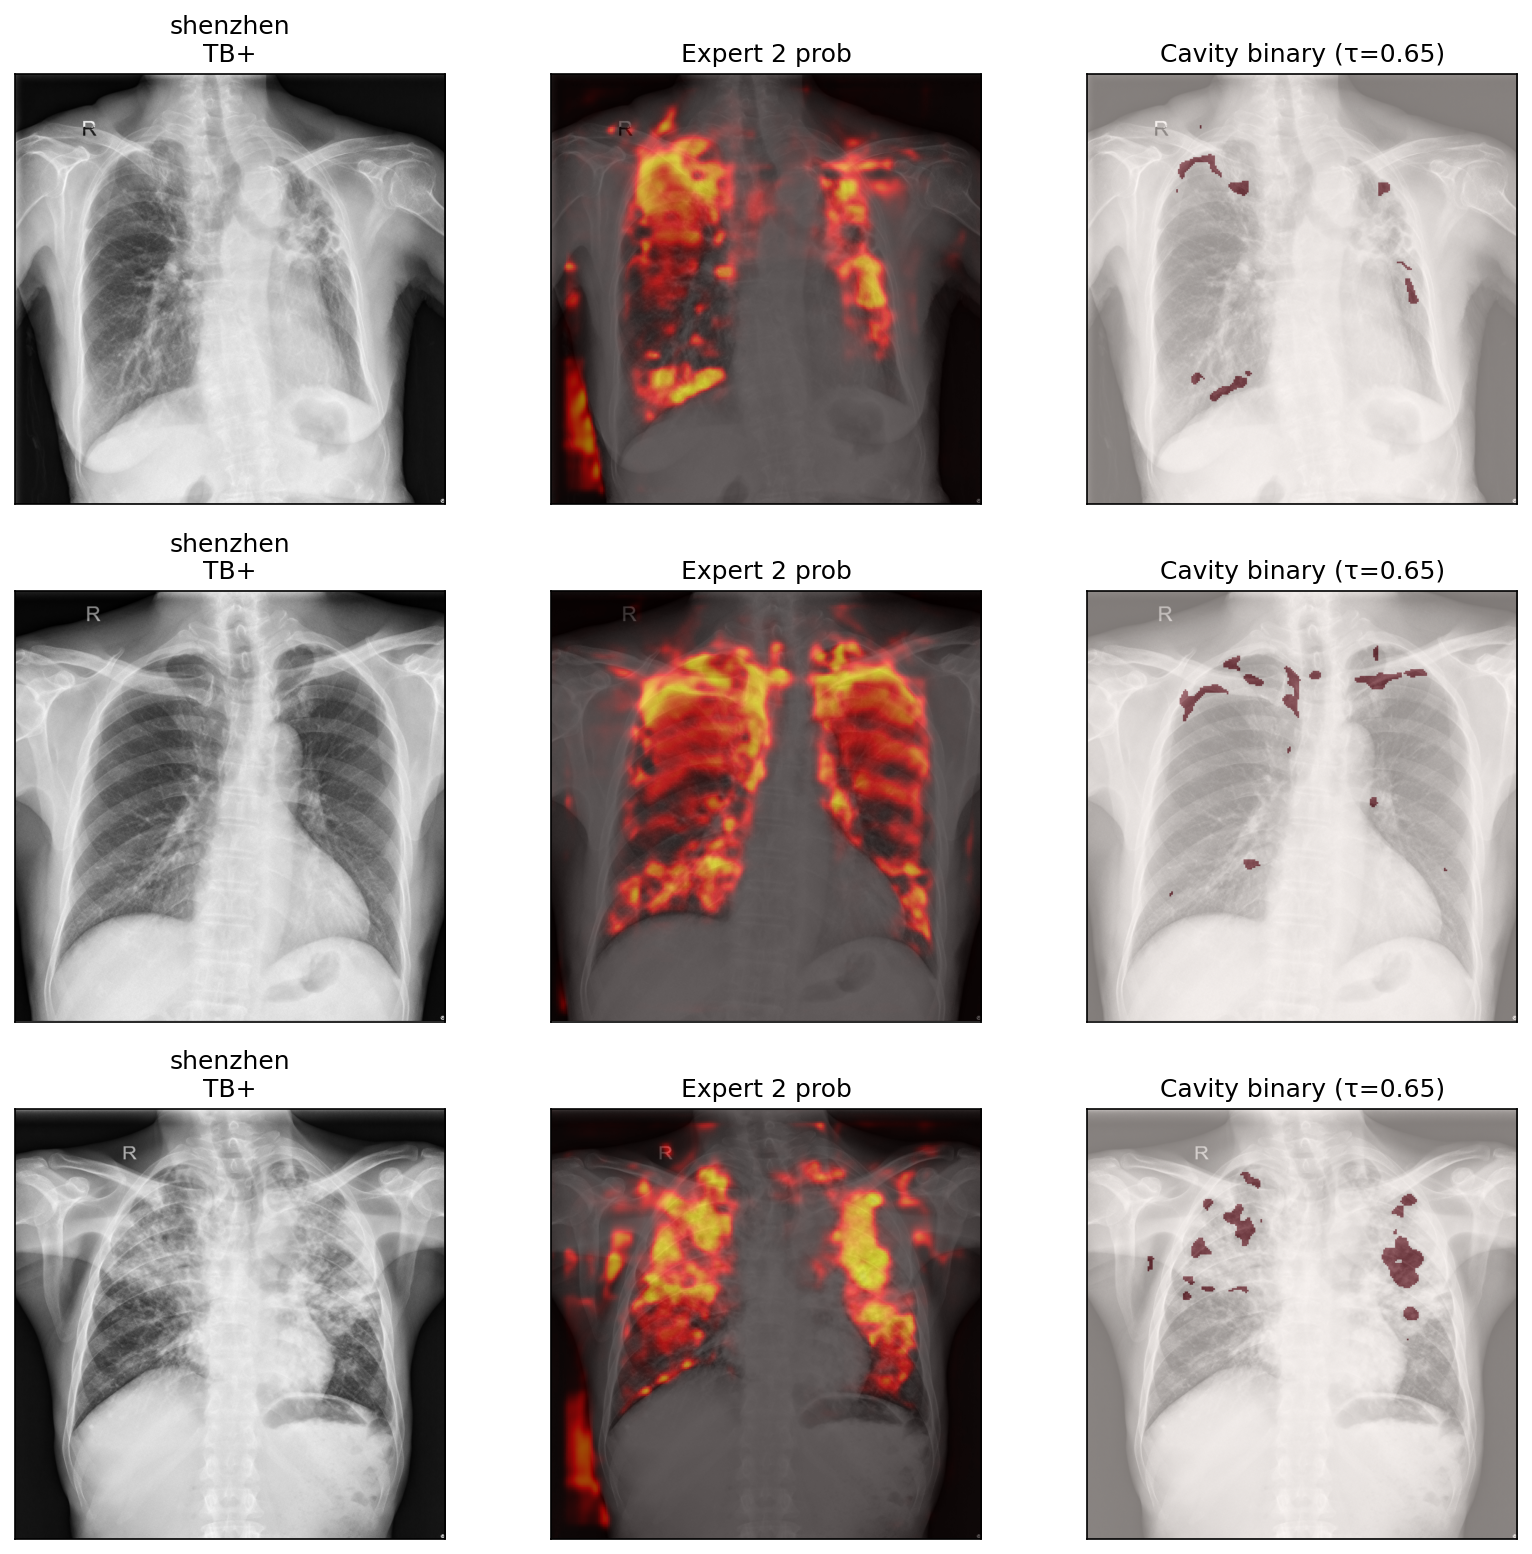
\includegraphics[width=0.95\columnwidth,height=0.22\textheight,keepaspectratio]{cavity_detection.png}
\caption{Cavity detection on three Shenzhen TB-positive cases. Columns: CXR, Expert\,2 cavity probability (heat), cavity binary mask at $\tau_{\text{cav}} = 0.65$. The probability maps localise air-space-like regions in the upper-zone parenchyma, the canonical cavitation distribution.}
\label{fig:cavity}
\end{figure}

Two stable regimes emerge. At $\tau_{\text{cav}} = 0.85$ Expert\,2 effectively never fires; Timika collapses to ALP-only and discrimination is high (0.741). At $\tau_{\text{cav}} = 0.55$ Expert\,2 fires for nearly all TB-positive cases (96.8\%); the $+40$ bonus is added almost uniformly across TB-positive predictions and discrimination is again strong (0.728). \emph{Between} these regimes, at the production $\tau_{\text{cav}} = 0.65$, Expert\,2 fires inconsistently (69.3\%): some TB+ cases receive the bonus and some do not, on no clinically meaningful basis given the absence of cavity ground truth. This stochastic application of a 40-point offset destroys the rank ordering and depresses Timika AUROC by roughly 13\,pp relative to either stable regime.

\textbf{Implication.} Expert\,2 is currently trained on pseudo-labels (consolidation-mask negatives within the lung field), not on radiologist cavity annotations. The training-data limitation manifests precisely as the intermediate-threshold collapse: the network has learned a smooth probability surface but lacks the calibrated decision boundary that explicit cavity supervision would provide. The ablation thereby converts an apparent hyperparameter sensitivity into a concrete scientific claim. Acquiring even a small cavity-annotated subset (for example, 100--200 cavity-rich Shenzhen images) is the single highest-impact future-work lever for this pipeline, expected to unlock the full discriminative power of the Timika $+40$ bonus.

\FloatBarrier
\section{Failure Cases}
\label{sec:failures}

Figure~\ref{fig:failure} highlights two characteristic failure modes. On an NIH-CXR14 case the lung mask spills outside the chest cavity, leading to a large MoE false-positive lesion. On a Montgomery case the lung mask is truncated at the lower border, producing edge-noise lesions. Both failure modes trace upstream to Component\,4 (lung segmentation) rather than to the lesion decoder itself, and they isolate a clear remediation path: improving lung-segmentation robustness on out-of-distribution acquisitions would propagate directly to the ALP and Timika outputs.

\begin{figure}[!htbp]
\centering
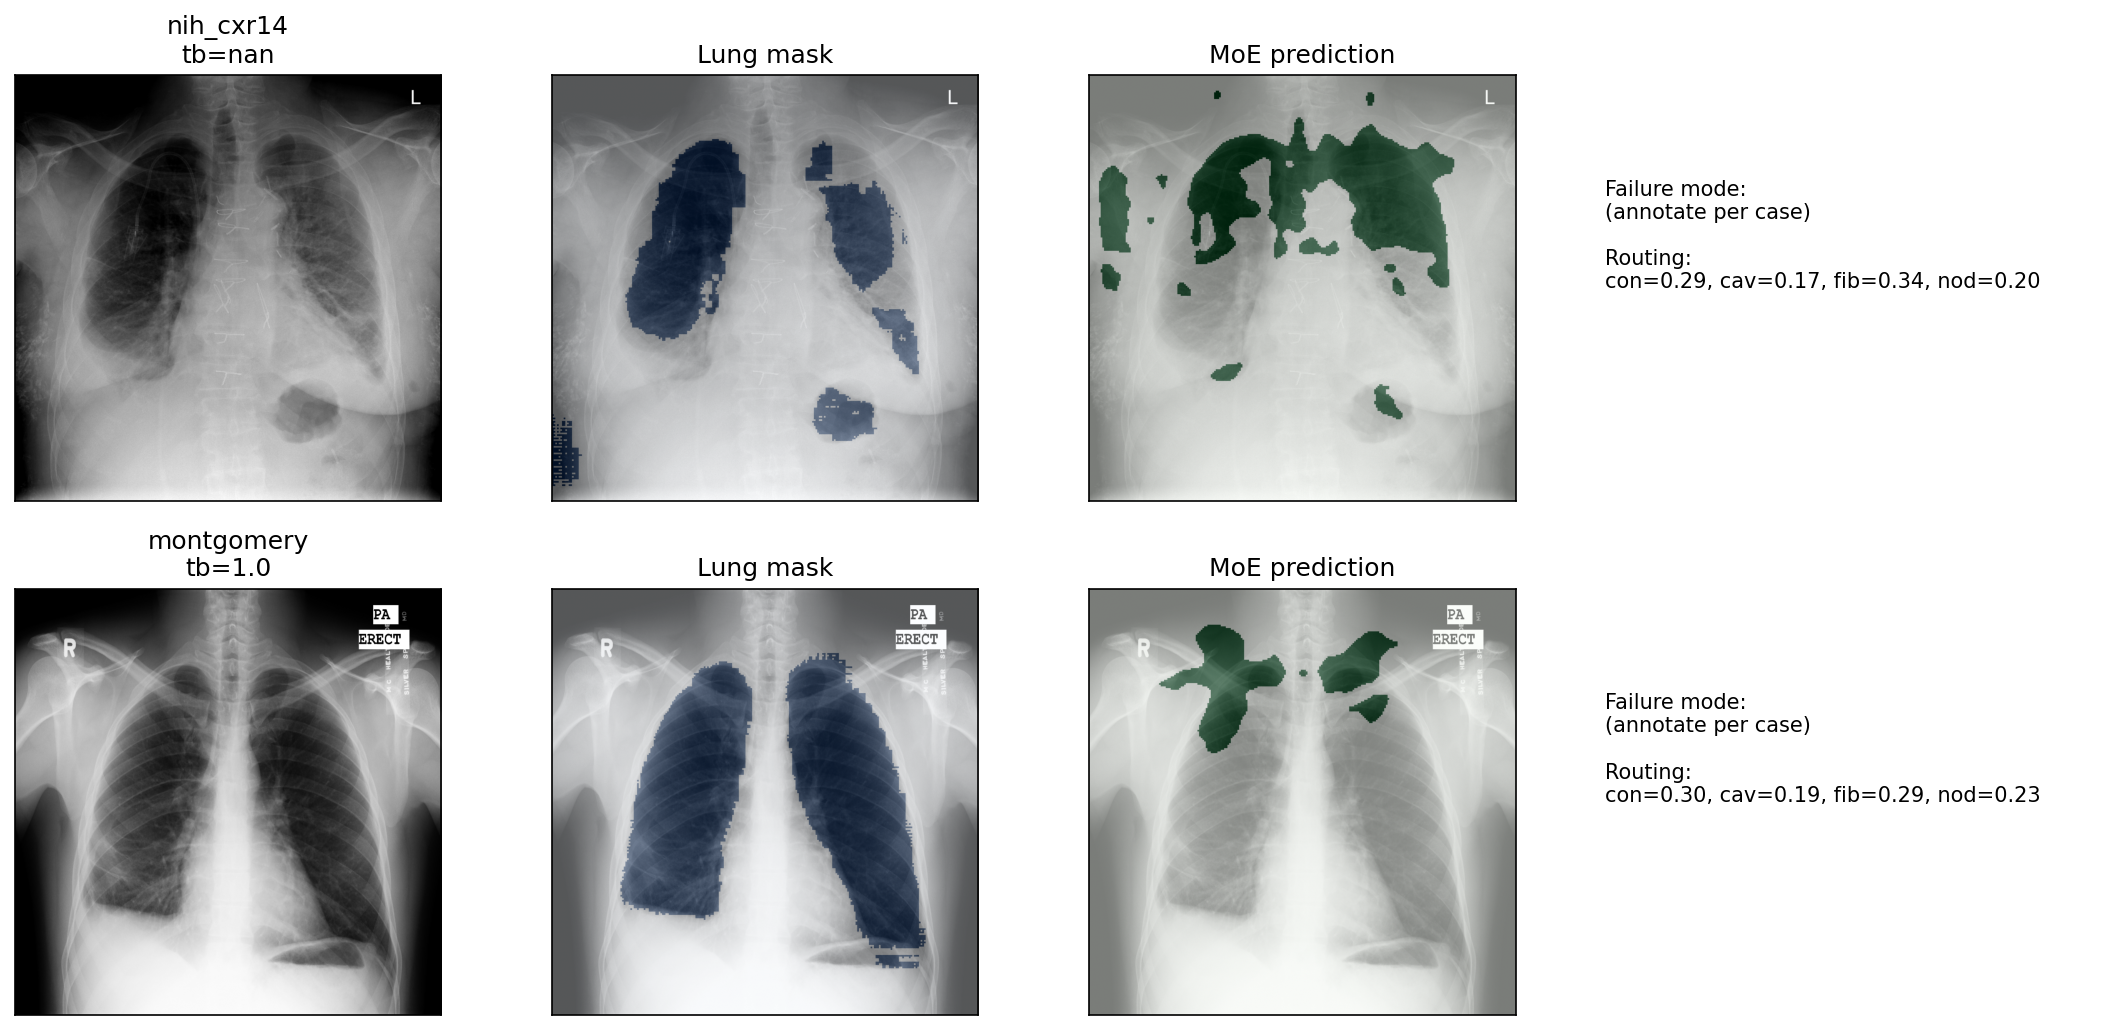
\includegraphics[width=0.95\columnwidth,height=0.22\textheight,keepaspectratio]{failure_cases.png}
\caption{Failure cases. Left: an NIH-CXR14 case where the lung mask spills outside the chest cavity, leading to a large MoE false-positive lesion. Right: a Montgomery case where the lung mask is truncated at the lower border, producing edge-noise lesions.}
\label{fig:failure}
\end{figure}

\FloatBarrier
\section{Discussion}
\label{sec:discussion}

\textbf{Headline ablation insight.} Section~\ref{sec:abl_C} identifies a non-monotonic response of Timika AUROC to the cavity binarisation threshold, with two stable regimes (no firing: 0.741; near-universal firing: 0.728) separated by a 13\,pp dip at the production threshold (0.613). This is a direct fingerprint of the underlying training-data limitation: Expert\,2 is trained on pseudo-labels rather than radiologist cavity annotations, so its decision boundary is uncalibrated. The ablation converts an apparent hyperparameter sensitivity into a concrete, actionable scientific claim about what supervision the system most needs.

\textbf{Limitations.} Four limitations bound the current results. First, the DANN domain classifier exhibits degeneracy and converges to predict TBX11K for the majority of inputs (35.7\% domain accuracy versus the 25\% target for full domain invariance). Second, Montgomery evaluation suffers from extreme variance ($n=28$, $\pm 0.19$ AUROC std), placing both Timika AUROCs within the noise floor on this dataset. Third, on TBX11K the MoE Timika AUROC (0.410) underperforms the baseline (0.774); TBX11K has the lowest cavitation prevalence (Expert\,2 fires on only 21.4\% of TB+ cases), so the cavity bonus introduces more noise than signal on this cohort. Fourth, the NIH ALP target ($\leq 10\%$) is not met (achieved 22.6\%), reflecting that the NIH pseudo-CAM training samples include non-TB pathology that contributes lesion-like activations. Hard-negative retraining with explicit healthy-image supervision is the indicated remedy.

\section{Conclusion}

We presented the first end-to-end automated pipeline for Timika severity scoring from chest X-rays, validated across four heterogeneous datasets. The four-expert Mixture-of-Experts lesion decoder delivers a Shenzhen Timika AUROC of 0.613 in production and 0.741 under the optimised cavity-threshold regime, alongside strong TB detection (overall AUROC 0.984) and lung segmentation ($+11$ Dice over MedSAM zero-shot). Three concrete future-work directions follow from the ablations, ranked by expected impact: (1) acquiring a small radiologist-annotated cavity dataset to resolve the intermediate-threshold collapse documented in Ablation\,C; (2) joint training of the gate and experts in a single phase; and (3) hardening Component\,4 against the lung-segmentation failure modes in Section~\ref{sec:failures}. The complete codebase, evaluation scripts, ablation harness, and trained checkpoints will be released upon acceptance to support reproducibility and clinical validation.

{\footnotesize
\bibliography{main}
\bibliographystyle{icml2021}
}

\end{document}
